\section{Second Exercise}
We have the identities
\begin{equation}
    X = HZH, \quad Y = iXZ.
\end{equation}
Then we have the hamiltonian 
\begin{equation}
    \mathcal{H} = X_1 \otimes Y_2 \otimes Z_3
\end{equation}
rewriting the Hamiltonian using the identities above we get
\begin{equation}
    \mathcal{H} = (H_1 Z_1 H_1) \otimes (i X_2 Z_2) \otimes Z_3
\end{equation}
which can be factored as
\begin{equation}
    \mathcal{H} =  (H_1 \otimes iX_2 \otimes \I) ( Z_1 \ot Z_2 \ot Z_3) (H_1 \ot \I \ot \I).
\end{equation}
From Nielsen \& Chuang we know that $\mathcal{H} = Z_1 \ot Z_2 \ot Z_3$ corresponds to Figure 4.19 in the book. Thus we need to apply the corresponding gates before and after this and we get
\begin{figure}[H]
    \centering
    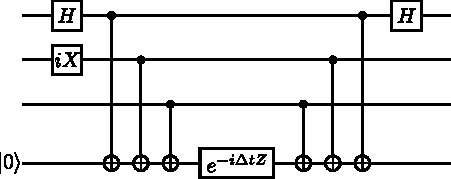
\includegraphics{figures/circuit_2.pdf}
\end{figure}